\section{Results Discussions}

The results obtained in the previous Chapter show that Service Restoration depends on the availability 
of transferring out-of-service un-faulted loads to healthy feeders, which in turn depends on the number 
and location of switches, i.e., if the location and number of switches are conducive, the SR algorithm 
can resupply all out-of-service un-faulted loads. 

Therefore, the SR algorithm obtained the optimal switch operations sequence for failure scenarios in 
which there was the possibility of transferring isolated loads to healthy feeders, and for those 
scenarios it restored all loads. 

The optimal sequence is obtained in the Training scenario but constantly updated in the Production
scenario. Consequently, the RL algorithm requires retraining when system variations occur that increase or 
reduce the numbers of lines or switches, but retraining is not required when these changes affect the 
number of loads. 

\subsection{SR Algorithm performance}
The performance of this algorithm relies on computational capacity: memory size and processing.

First, the RL model dictates the memory size required. This is because of the model needs to compute a Q 
Values matrix, whose size depends on the numbers of actions and states and, in turn, on the numbers of 
lines and switches, as explained in Chapter 3. Accordingly, Figure \ref{ch-conclusions:fig:memory} shows the amount of 
memory needed under the numbers of lines and switches for the IEEE 123 Node Test Feeder with 10 switches.
As a result, memory size grows linearly with an increase in the number of lines and exponentially with 
an increase in the number of switches. 
\begin{figure}[!ht]
    \centering
	\subfloat[Memory size according to number of switches ]{
        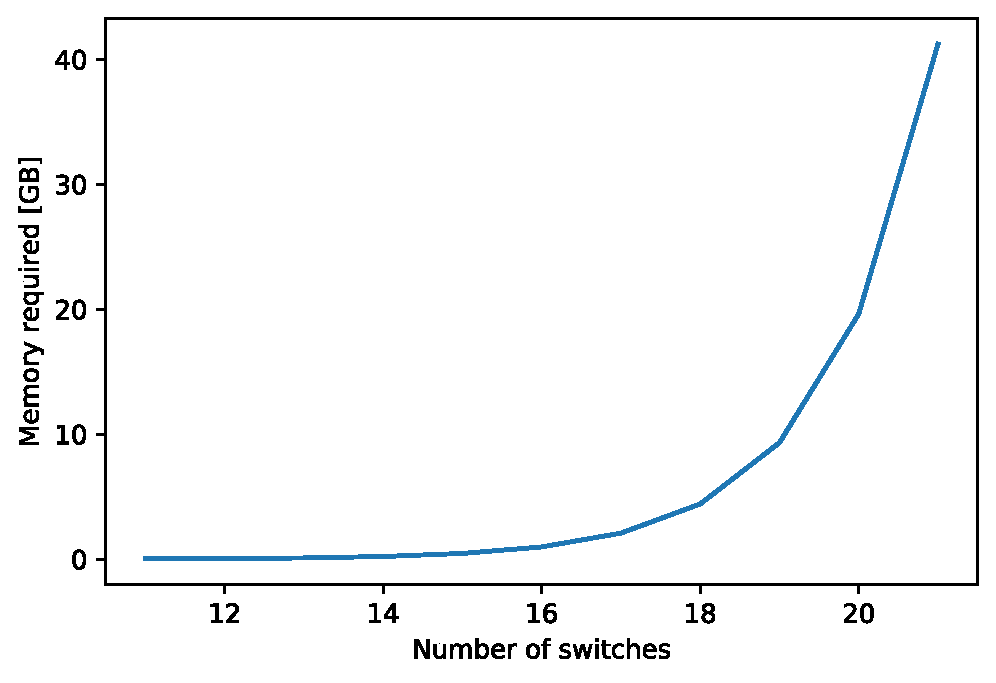
\includegraphics[scale=0.4]{_conclusions/fig/switches.pdf}
		\label{ch-conclusions:fig:ms_switches}
	}%
	\qquad
	\subfloat[Memory size according to number of lines]{
        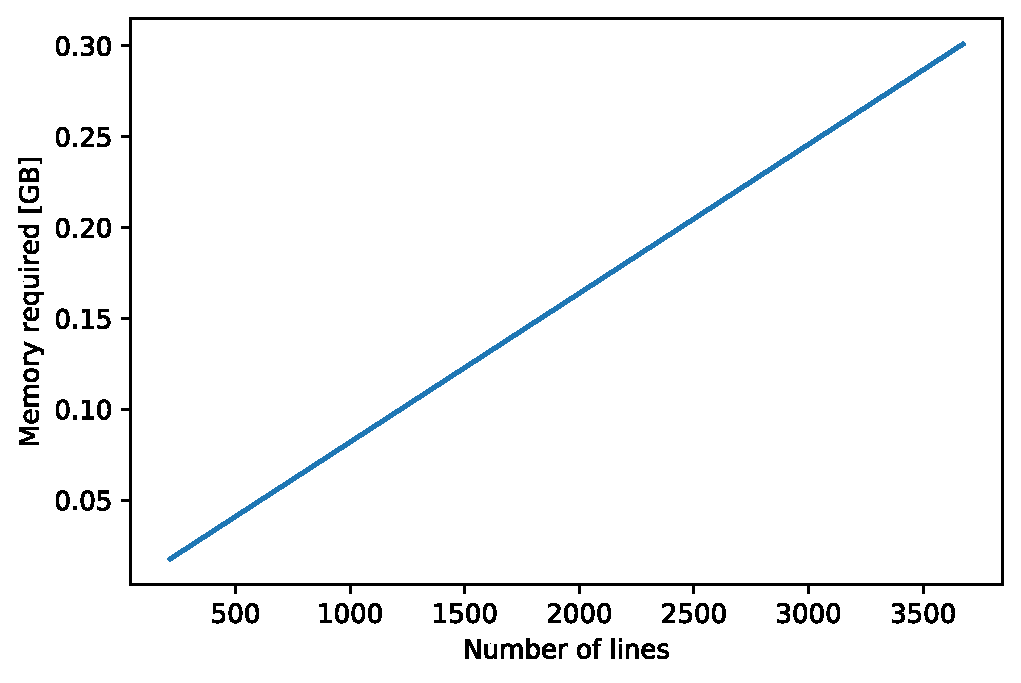
\includegraphics[scale=0.4]{_conclusions/fig/lines.pdf}
		\label{ch-conclusions:fig:ms_lines}
	}
	\caption{Memory size comparison according to numbers of lines and switches variations for the IEEE 123 Node Test Feeder - 10 switches}
	\label{ch-conclusions:fig:memory}	
\end{figure}


Since the number of switches is the factor that most affects the size of the model, Figure \ref{ch-conclusions:fig:123_swtimestates} 
presents the required processing time and the number of states according to the number of switches for the IEEE 123 Node Test Feeder.


\begin{figure}
    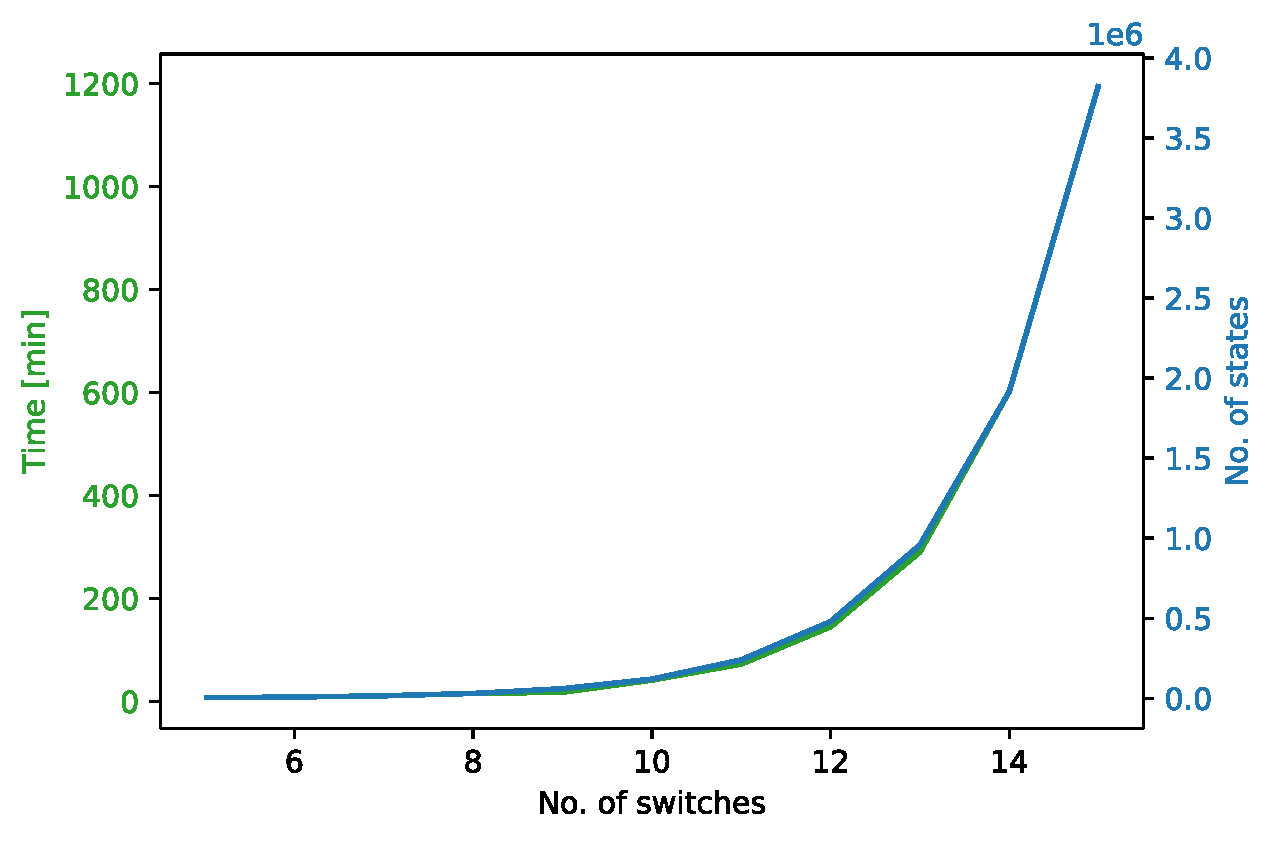
\includegraphics[scale=0.5]{_conclusions/fig/swtimestates.pdf}
    \centering
    \caption{No. of switches vs Time [min] and No. of states - IEEE 123 Node Test Feeder}
    \label{ch-conclusions:fig:123_swtimestates}
\end{figure}
\newpage 
\newpage
